\documentclass[12pt]{article}

% TeX calculates margins from a point 1 inch from the top and 1 inch
% from the left of the page. So the total left margin for instance is
% the 'oddsidemargin' + 1 inch.
%
%\setlength{\textwidth}{4.5in}
%\setlength{\textheight}{7.0in}
%\setlength{\evensidemargin}{0.0in}
%\setlength{\oddsidemargin}{0.0in}
%\setlength{\topmargin}{0.5in}

\usepackage{graphicx}
\usepackage{latexsym}
\usepackage{amsmath}
\usepackage{wrapfig}
\usepackage{algorithmic}
\usepackage[boxed]{algorithm}
\usepackage{rotating}
\usepackage{multicol}
%\usepackage{times}

%\displaybreak[0]       %% Break permitted but not encouraged

\begin{document}

\title{MSTK: Mesh Toolkit, v 1.1 - DRAFT} 


\author{Rao V. Garimella \\
  Mathematical Modeling and Analysis (T-7), Theoretical Division, \\
  Los Alamos National Laboratory, Los Alamos, NM, USA. \\ E-mail:
  rao@lanl.gov}

\maketitle

\thispagestyle{empty}
\setlength{\parindent}{0.0in}
\setlength{\parskip}{0.5em}

\newpage
\section{Introduction}

MSTK or Mesh Toolkit is a mesh framework that allows users to
represent, manipulate and query unstructured 3D arbitrary topology
meshes in a general manner without the need to code their own data
structures. MSTK is a flexible framework in that it allows (or will
eventually allow) a wide variety of underlying representations for the
mesh while maintaining a common interface. It will allow users to
choose from different mesh representations either at initialization or
during the program execution so that the optimal data structures are
used for the particular algorithm. The interaction of users and
applications with MSTK is through a functional interface that acts as
though the mesh always contains vertices, edges, faces and regions and
maintains connectivity between all these entities.

\par MSTK allows for the simultaneous existence of an arbitrary number of
meshes. However, any entity in MSTK can belong to only one mesh at a
time.

\par MSTK will eventually support distributed meshes for parallel
computing. However, this is still not in place.

\par MSTK will soon allow applications to attach application or field data
to entities. This data may be integers, reals (doubles), integer
vectors, real (double) vectors, integer tensors, real (double tensors)
and pointers. 

\par The basis for development of MSTK is laid out in the following paper:

Garimella, R. ``Mesh Data Structure Selection for Mesh Generation and
FEA Applications,'' \textit{International Journal of Numerical Methods
  in Engineering}, v55 n4, pp. 441-478, 2002.

In the following sections, the data types of MSTK will be described
followed by a description of the functional interface. The MSTK file
format will be described in the last section.

\newpage
\section{MSTK Data Types}

\begin{description}
\item[]\textbf{\textit{Set\_ptr}}: Handle to a Set object

\item[]\textbf{\textit{Mesh\_ptr}}: Handle to a Mesh object.

\item[]\textbf{\textit{MVertex\_ptr}}: Handle to a Mesh Vertex object (Topological
Dimension 0)

\item[]\textbf{\textit{MEdge\_ptr}}: Handle to a Mesh Edge object (Topological Dimension 1)

\item[]\textbf{\textit{MFace\_ptr}}: Handle to a Mesh Face object (Topological Dimension 2)

\item[]\textbf{\textit{MRegion\_ptr}}: Handle to Mesh Region object (Topological Dimension 3)

\item[]\textbf{\textit{MEntity\_ptr}}: Handle to a generic Mesh Entity object. Any of
the above types of entities can be cast as \textit{MEntity\_ptr}

\item[]\textbf{\textit{GModel\_ptr}}: Handle to a Geometric Model object
\item[]\textbf{\textit{GEntity\_ptr}}: Handle to a Geometric Entity object

  
\item[]\textbf{\textit{RepType}}: Enumerated type describing the type
  of mesh representation.  Can be UNKNOWN\_REP, F1, F4, R1, R2, R4.
  See Appendix~\ref{app:reptypes} for schematics of these
  representations \textit{Currently only representation types F1 and
    F4 are supported}

\item[]\textbf{\textit{MFType}}: Enumerated type for mesh face type
Can be FDELETED, FUNKNOWN, TRI, QUAD, POLYGON

\item[]\textbf{\textit{MRType}}: Enumerated type for mesh region type
Can be RDELETED, RUNKNOWN, TET, PYRAMID, PRISM, HEX, POLYHED
\end{description}

\newpage
\section{MSTK Functional Interface}
\subsection{Sets}

Sets of entities in MSTK are returned as sets of type
\textit{Set\_ptr}. The following are the set operations available in
MSTK:

\begin{description}
\item[]\textbf{\textit{Set\_ptr} Set\_New(\textit{int} inisize):} Create a
new set with an initial size, \textit{inisize}. If \textit{inisize} is
0, the initial size is set to be 10.

\item[]\textbf{\textit{void} Set\_Delete(\textit{Set\_ptr} l):} Delete a set.

\item[]\textbf{\textit{Set\_ptr} Set\_Compress(\textit{Set\_ptr} l):} Compress
a set.  Doing this while an algorithm is iterating through the set can
currently cause problems!! Calling \textbf{Set\_Compress} could change the
pointer for the set due to reallocation.

\item[]\textbf{\textit{Set\_ptr} Set\_Copy(\textit{Set\_ptr} l):} Return a
copy of a set.

\item[]\textbf{\textit{Set\_ptr} Set\_Add(\textit{Set\_ptr} l, \textit{void
  *}entry):} Add an entry to the set. The entry is appended to the end
of the set.

\item[]\textbf{\textit{Set\_ptr} Set\_ChknAdd(\textit{Set\_ptr} l,
\textit{void *}entry):} Add an entry to a set only if it is not already
in the set.

\item[]\textbf{\textit{int} Set\_Rem(\textit{Set\_ptr} l, \textit{void
  *}entry):} Remove an entry from the set. Returns 1 if successful, 0
otherwise.

\item[]\textbf{\textit{int} Set\_Remi(\textit{Set\_ptr} l, \textit{int} i):}
Remove the i'th valid entry in the set. Returns 1 if successful, 0
otherwise.

\item[]\textbf{\textit{int} Set\_Replace(\textit{Set\_ptr} l, \textit{void
  *}entry, \textit{void *}nuentry):} Replace 'entry' with 'nuentry' in
set. Returns 1 if successful, 0 otherwise.

\item[]\textbf{\textit{int} Set\_Replacei(\textit{Set\_ptr} l, \textit{int}
i, void *nuentry):} Replace the i'th valid entry in the set with
'nuentry'. Returns 1 if successful, 0 otherwise.

\item[]\textbf{\textit{int} Set\_Contains(\textit{Set\_ptr} l, void *entry):}
Returns 1 if set contains the entry, 0 otherwise.

\item[]\textbf{\textit{int} Set\_Locate(\textit{Set\_ptr} l, void *entry):}
Returns the positional index of the entry in the set. Returns -1 if
the set does not contain the entry.

\item[]\textbf{\textit{void *}Set\_Entry(\textit{Set\_ptr} l, \textit{int}
i):} Return the i'th valid entry in the set.  Returns a NULL pointer if
the i'th valid entry could not be found.

\item[]\textbf{\textit{void *}Set\_Next\_Entry(\textit{Set\_ptr} l,
\textit{int} *i):} Return the next valid entry in the set. This routine
works like an iterator. To start iterating through the set, set the
iteration index i=0 and call the routine to get the first entry in the
set. Subsequent calls to the routine will iterate through the entries
in the set. The routine will return a NULL to indicate that the end of
the set is reached.

The value of the iteration index i will be modified by the routine on
each call to indicate where in the set it is. This value should not be
modified externally while iterating through the set. Also, no specific
meaning be derived from from the iteration index by other applications
since the internal implementation and interpretation of the index may
change at any time.

\item[]\textbf{\textit{int} Set\_Num\_Entries(\textit{Set\_ptr} l):} Return
the number of entries in a set
\end{description}

\newpage
\subsection{Mesh Object}

A mesh object is a set of vertices (nodes) possibly connected by other
entities such as edges, faces, regions. Depending on the
representation chosen and type of mesh, some or all of the entities
may be explicitly stored.  Full representations contain all types of
entities up to the highest dimension of the mesh. For example, a full
representation of a tetrahedral mesh contains vertices, edges, faces
and regions. However, one type of reduced representation of this mesh
may contain only vertices and regions. For a surface mesh, a full
representation includes vertices, edges and faces while a reduced
representation only has vertices and faces. Also, depending on the
type of representation, some adjacencies (information about which
entities are connected to which other entities) are stored and others
are derived.

 
\begin{description}
\item[]\textbf{\textit{Mesh\_ptr} MESH\_New(\textit{RepType} type):}
Initialize a new mesh object with the given representation type which
can be F1, F2, F3, F4, F5, F6, R1, R2, R3, R4. Not all of these types
are implemented. If the representation type is not known at the
present time (e.g. before reading the mesh from a file), the
representation type of UNKNOWN\_REP can be specified.  Note that this
only initializes a mesh object, it does not create or generate a mesh
which is the work of high level mesh generation routines.

\item[]\textbf{\textit{int} MESH\_InitFromFile(\textit{Mesh\_ptr} mesh,
const char *filename):} Initialize or read a mesh from file into the
given mesh object. Returns 1 if successful, 0 otherwise.

\item[]\textbf{\textit{void} MESH\_WriteToFile(\textit{Mesh\_ptr} mesh,
const char *filename):} Save a mesh to a filename. The file is created
if it does not exists. It is recommended that the .mstk extension be
used for MSTK mesh files.  However, there is no such requirement.

\item[]\textbf{\textit{GModel\_ptr} MESH\_GModel(\textit{Mesh\_ptr} mesh):}
Return a handle to the underlying geometric model. If there is no
geometric model associated with the mesh, NULL pointer is returned.

\item[]\textbf{\textit{RepType} MESH\_RepType(\textit{Mesh\_ptr} mesh):}
Representation type currently being used by the mesh.

\item[]\textbf{\textit{int} MESH\_Num\_Vertices(\textit{Mesh\_ptr} mesh):}
Number of vertices in the mesh.

\item[]\textbf{\textit{int} MESH\_Num\_Edges(\textit{Mesh\_ptr} mesh):}
Number of edges in the mesh. For reduced representations, this routine
returns 0 since it is impractically expensive to count the number of
edges when they do not explicitly exist. Applications must find a way
to avoid using this routine for reduced representations.

\item[]\textbf{\textit{int} MESH\_Num\_Faces(\textit{Mesh\_ptr} mesh):}
Number of faces in the mesh. For reduced representations R1 or R2,
this routine counts only the faces that are explicitly represented
i.e. faces not connected to any mesh region. Therefore, a value of 0
will be returned for the number of faces of a tetrahedral mesh with
representation R1 or R2 but the correct number will be reported for a
tetrahedral mesh in other representations. Also, the correct number
will be reported for the number of faces in a surface mesh in
representation R1 or R2.  Therefore, this routine must be used
carefully.


\item[]\textbf{\textit{int} MESH\_Num\_Regions(\textit{Mesh\_ptr} mesh):}
Number of regions in the mesh.


\item[]\textbf{\textit{MVertex\_ptr} MESH\_Vertex(\textit{Mesh\_ptr} mesh,
\textit{int} i):} Return the i'th vertex in the mesh. Returns NULL if i
$<$ 0 or i $>$ number of mesh vertices.

\item[]\textbf{\textit{MEdge\_ptr} MESH\_Edge(\textit{Mesh\_ptr} mesh,
\textit{int} i):} Return the i'th edge in the mesh. Returns NULL if i $<$
0 or i $>$ number of mesh edges. Returns NULL for reduced
representations.

\item[]\textbf{\textit{MFace\_ptr} MESH\_Face(\textit{Mesh\_ptr} mesh,
\textit{int} i):} Return the i'th face in the mesh. Returns NULL if i $<$
0 or i $>$ number of mesh faces. Only faces explicitly represented in
the mesh are returned for reduced representation (See explanation for
MESH\_Num\_Faces).

\item[]\textbf{\textit{MRegion\_ptr} MESH\_Region(\textit{Mesh\_ptr} mesh,
\textit{int} i):} Return the i'th region in the mesh. Returns NULL if i
$<$ 0 or i $>$ number of mesh region.


\item[]\textbf{\textit{MVertex\_ptr} MESH\_Next\_Vertex(\textit{Mesh\_ptr}
mesh, \textit{int} *idx):} Returns the next vertex while iterating
through the vertices of the mesh. See the routine \textbf{Set\_Next\_Entry}
above for an explanation of how the iteration works.

\item[]\textbf{\textit{MEdge\_ptr} MESH\_Next\_Edge(\textit{Mesh\_ptr} mesh,
\textit{int} *idx):} Returns the next edge while iterating through the
edges of the mesh. See the routine Set\_Next\_Entry above for an
explanation of how the iteration works.  The routine always returns
NULL for reduced representations.


\item[]\textbf{\textit{MFace\_ptr} MESH\_Next\_Face(\textit{Mesh\_ptr} mesh,
\textit{int} *idx):} Returns the next face while iterating through the
faces of the mesh. See the routine \textbf{Set\_Next\_Entry} above for
an explanation of how the iteration works.  Only faces explicitly
represented in the mesh are returned for reduced representation (See
explanation for \textbf{MESH\_Num\_Faces}).


\item[]\textbf{\textit{void} MESH\_Add\_Vertex(\textit{Mesh\_ptr} mesh,
\textit{MVertex\_ptr} v):} Add a vertex to the mesh. It is assumed that
the vertex and its coordinates set are properly defined.

\item[]\textbf{\textit{void} MESH\_Add\_Edge(\textit{Mesh\_ptr} mesh,
\textit{MEdge\_ptr} e):} Add an edge to the mesh. It is assumed that
the edge is and its topology is defined.

\item[]\textbf{\textit{void} MESH\_Add\_Face(\textit{Mesh\_ptr} mesh,
\textit{MFace\_ptr} f):} Add a face to the mesh. It is assumed that the
face and its topology is properly defined.

\item[]\textbf{\textit{void} MESH\_Add\_Region(\textit{Mesh\_ptr} mesh,
\textit{MRegion\_ptr} r):} Add a region to the mesh. It is assumed that
the region and its topology is properly defined.

\item[]\textbf{\textit{void} MESH\_Rem\_Vertex(\textit{Mesh\_ptr} mesh,
\textit{MVertex\_ptr} v):} Remove vertex from mesh. Vertex is not
deleted and must be deleted afterward separately.

\item[]\textbf{\textit{void} MESH\_Rem\_Edge(\textit{Mesh\_ptr} mesh,
\textit{MEdge\_ptr} e):} Remove edge from mesh. Edge is not deleted and
must be deleted afterward separately.

\item[]\textbf{\textit{void} MESH\_Rem\_Face(\textit{Mesh\_ptr} mesh,
\textit{MFace\_ptr} f):} Remove face from mesh. Face is not deleted and
must be deleted afterward separately.

\item[]\textbf{\textit{void} MESH\_Rem\_Region(\textit{Mesh\_ptr} mesh,
\textit{MRegion\_ptr} r):} Remove region from mesh. Region is not deleted and must be deleted afterward separately.

\item[]\textbf{\textit{void} MESH\_Set\_GModel(\textit{Mesh\_ptr} mesh,
GModel\_ptr geom):} Assign a geometric model handle to the mesh.

\item[]\textbf{\textit{int} MESH\_Change\_RepType(\textit{Mesh\_ptr} mesh,
\textit{int} nurep):} Change the representation type of the mesh. This
routine can be used to modify the representation type dynamically to
suit different algorithms.  However, the cost of making the change and
reordering all adjacencies and creating or deleting entities has to be
considered while invoking this routine. Also, once a conversion is
made from a full representation to a reduced representation, not all
information may be retrievable when switching back to a full
representation.  (particularly classification information, i.e.,
relationship of mesh entities to the geometric model).

\end{description}

\newpage
\subsection{Mesh Vertex Object}

\begin{description}
\item[]\textbf{\textit{MVertex\_ptr} MV\_New(\textit{Mesh\_ptr} mesh):}
Create a new vertex object. No geometric or topological information is
embedded in the vertex when it is created. The vertex only knows which
mesh it belongs to. The ID of the vertex is set by this function.

\item[]\textbf{\textit{void} MV\_Delete(\textit{MVertex\_ptr} mvertex):}
Delete the vertex. Deletes all topological and geometric
information embedded in the vertex.

\item[]\textbf{\textit{void} MV\_Set\_Coords(\textit{MVertex\_ptr} mvertex,
double *xyz):} Set the coordinates of the vertex.

\item[]\textbf{\textit{void} MV\_Set\_GEntity(\textit{MVertex\_ptr} mvertex,
GEntity\_ptr gent):} Set the geometric model entity on which vertex is
classified.


\item[]\textbf{\textit{void} MV\_Set\_GEntDim(\textit{MVertex\_ptr} mvertex,
\textit{int} gdim):} Set topological dimension of model entity on which
vertex is classified.

\item[]\textbf{\textit{void} MV\_Set\_GEntID(\textit{MVertex\_ptr} mvertex,
\textit{int} gid):} Set ID of model entity on which vertex is
classified.

\item[]\textbf{\textit{void} MV\_Add\_AdjVertex(\textit{MVertex\_ptr}
mvertex, \textit{MVertex\_ptr} adjvertex):} Add neighboring vertex,
adjvertex, to ajdacent vertex list of vertex, mvertex.

\item[]\textbf{\textit{void} MV\_Rem\_AdjVertex(\textit{MVertex\_ptr}
mvertex, \textit{MVertex\_ptr} adjvertex):} Delete neighboring vertex
of given vertex.

\item[]\textbf{\textit{void} MV\_Set\_ID(\textit{MVertex\_ptr} mvertex,
\textit{int} id):} Explicitly set ID of a vertex and overwrite the ID
set by the MV\_New operator. Does not check for duplication of edge
IDs.

\item[]\textbf{\textit{Mesh\_ptr} MV\_Mesh(\textit{MVertex\_ptr} mv):}
Returns the mesh that this vertex belongs to.

\item[]\textbf{\textit{int} MV\_ID(\textit{MVertex\_ptr} mvertex):} Returns
the ID of the vertex. 

\item[]\textbf{\textit{int} MV\_GEntDim(\textit{MVertex\_ptr} mvertex):}
Returns the dimension of the geometric model entity that the vertex is
classified on. Returns -1 if not known.

\item[]\textbf{\textit{int} MV\_GEntID(\textit{MVertex\_ptr} mvertex):}
Returns the ID of the geometric model entity that the vertex is
classified on. Returns 0 if this information is not known.

\item[]\textbf{\textit{GEntity\_ptr} MV\_GEntity(\textit{MVertex\_ptr}
  mvertex):} Returns a pointer or handle to the geometric model entity
  that the vertex is classified on. Returns NULL if this information
  is not known.

\item[]\textbf{\textit{void} MV\_Coords(\textit{MVertex\_ptr} mvertex,
double *xyz):} Returns the coordinates of the vertex.


\item[]\textbf{\textit{int} MV\_Num\_AdjVertices(\textit{MVertex\_ptr}
mvertex):} Returns the number of edge connected neighboring vertices of
vertex. \textit{Not efficient for all representations}.

\item[]\textbf{\textit{int} MV\_Num\_Edges(\textit{MVertex\_ptr} mvertex):}
Returns the number of edges connected to the vertex.

\item[]\textbf{\textit{int} MV\_Num\_Faces(\textit{MVertex\_ptr} mvertex):}
Returns the number of faces connected to the vertex.

\item[]\textbf{\textit{int} MV\_Num\_Regions(\textit{MVertex\_ptr} mvertex):}
Returns the number of regions connected to the vertex

\item[]\textbf{\textit{Set\_ptr} MV\_AdjVertices(\textit{MVertex\_ptr}
mvertex):} Set of adjacent or edge connected neighboring vertices of vertex.

\item[]\textbf{\textit{Set\_ptr} MV\_Edges(\textit{MVertex\_ptr} mvertex):}
Set of edges connected to the vertex.

\item[]\textbf{\textit{Set\_ptr} MV\_Faces(\textit{MVertex\_ptr} mvertex):}
Set of faces connected to the vertex.

\item[]\textbf{\textit{Set\_ptr} MV\_Regions(\textit{MVertex\_ptr} mvertex):}
Set of regions connected to the vertex.
\end{description}



\newpage
\subsection{Mesh Edge Object}

\begin{description}
\item[]\textbf{\textit{MEdge\_ptr} ME\_New(\textit{Mesh\_ptr} mesh):} Create
a new edge object. No topological information is embedded in the edge
when it is created. The edge only knows which mesh it belongs
to. The ID of the edge is set by this function.

\item[]\textbf{\textit{void} ME\_Delete(\textit{MEdge\_ptr} medge):} Delete
the edge. Deletes all topological information embedded in the edge.

\item[]\textbf{\textit{void} ME\_Set\_GEntity(\textit{MEdge\_ptr} medge,
GEntity\_ptr gent):} Set the geometric model entity on which the edge
is classified.

\item[]\textbf{\textit{void} ME\_Set\_GEntDim(\textit{MEdge\_ptr} medge,
\textit{int} gdim):} Set the topological dimension of model entity on
which edge is classified.

\item[]\textbf{\textit{void} ME\_Set\_GEntID(\textit{MEdge\_ptr} medge,
\textit{int} gid):} Set ID of model entity on which edge is classified.

\item[]\textbf{\textit{void} ME\_Set\_ID(\textit{MEdge\_ptr} medge,
\textit{int} id):} Explicitly set ID of an edge and overwrite the ID set
by the ME\_New function. Does not check for duplication of edge IDs.

\item[]\textbf{\textit{void} ME\_Set\_Vertex(\textit{MEdge\_ptr} medge,
\textit{int} i, \textit{MVertex\_ptr} vertex):} Set the i'th vertex of
the edge. i can be 0 or 1.

\item[]\textbf{\textit{void} ME\_Replace\_Vertex(\textit{MEdge\_ptr} medge,
\textit{MVertex\_ptr} vert, \textit{MVertex\_ptr} nuvert):} Replace
i'th vertex by new vertex.

\item[]\textbf{\textit{Mesh\_ptr} ME\_Mesh(\textit{MEdge\_ptr} medge):}
Returns the mesh that this edge belongs to.

\item[]\textbf{\textit{int} ME\_ID(\textit{MEdge\_ptr} medge):} Returns the
ID of the vertex. Returns -1 if not known.

\item[]\textbf{\textit{int} ME\_GEntDim(\textit{MEdge\_ptr} medge):} Returns
the dimension of the geometric model entity that the vertex is
classified on. Returns -1 if not known.

\item[]\textbf{\textit{int} ME\_GEntID(\textit{MEdge\_ptr} medge):} Returns
the ID of the geometric model entity that the vertex is classified on.
Returns 0 if this information is not known.

\item[]\textbf{\textit{GEntity\_ptr} ME\_GEntity(\textit{MEdge\_ptr} medge):} Returns
a pointer or handle to the geometric model entity that the vertex is
classified on. Returns NULL if this information is not known.

\item[]\textbf{\textit{int} ME\_Num\_Faces(\textit{MEdge\_ptr} medge):}
Returns the number of faces connected to the edge.

\item[]\textbf{\textit{int} ME\_Num\_Regions(\textit{MEdge\_ptr} medge):}
Returns the number of regions connected to the edge.

\item[]\textbf{\textit{MVertex\_ptr} ME\_Vertex(\textit{MEdge\_ptr} medge,
\textit{int} i):} Returns the i'th vertex of the edge. i=0 returns the
first vertex and i=1 returns the second vertex.

\item[]\textbf{\textit{MVertex\_ptr} ME\_OppVertex(\textit{MEdge\_ptr}
medge, \textit{MVertex\_ptr} ov):} Return the vertex opposite to given
vertex in edge.

\item[]\textbf{\textit{int} ME\_UsesEntity(\textit{MEdge\_ptr} medge,
\textit{MEntity\_ptr} mentity, \textit{int} etype):} Check if edge uses
given lower dimension entity, \textit{mentity}. The dimension of the
entity is specified by the \textit{etype} variable. For an edge, the
only lower dimensional entity is a vertex. If the edge uses the
vertex, the function returns 1; otherwise it returns 0. If any
other type of entity is specified, the function returns 0.


\item[]\textbf{\textit{Set\_ptr} ME\_Faces(\textit{MEdge\_ptr} medge):}
Returns the set of faces using this edge.

\item[]\textbf{\textit{Set\_ptr} ME\_Regions(\textit{MEdge\_ptr} medge):}
Returns the set of regions using this edge.


\item[]\textbf{\textit{MEdge\_ptr} MVs\_CommonEdge(\textit{MVertex\_ptr} v1,
\textit{MVertex\_ptr} v2):} Return the edge connecting vertices v1 and
v2, if it exists. If such an edge does not exist, the function returns
0.

\item[]\textbf{\textit{double} ME\_Len(\textit{MEdge\_ptr} e):} Return
  the length of the straight line connecting the two vertices of the
  edge.

\item[]\textbf{\textit{double} ME\_LenSqr(\textit{MEdge\_ptr} e):}
  Return the square of the length of the straight line connecting the
  two vertices of the edge.

\item[]\textbf{\textit{void} ME\_Vec(\textit{MEdge\_ptr} e, double *evec):}
Return the vector going from the first vertex of the edge to the
second vertex of the edge.
\end{description}



\newpage
\subsection{Mesh Face Object}

\begin{description}
\item[]\textbf{\textit{MFace\_ptr} MF\_New(\textit{Mesh\_ptr} mesh):} Create
a new face object. No topological information is embedded in the face
when it is created. The face only knows which mesh it belongs
to. The ID of the face is set by this function.

\item[]\textbf{\textit{void} MF\_Delete(\textit{MFace\_ptr} mface):} Delete
the face. Delete all topological information embedded in the face.

\item[]\textbf{\textit{void} MF\_Set\_GEntity(\textit{MFace\_ptr} mface, GEntity\_ptr gent):} Set the geometric model entity on which the edge is classified.

\item[]\textbf{\textit{void} MF\_Set\_GEntDim(\textit{MFace\_ptr} mface,
\textit{int} gdim):} Set the dimension of the geometric model entity on
which the face is classified.

\item[]\textbf{\textit{void} MF\_Set\_GEntID(\textit{MFace\_ptr} mface,
\textit{int} gid):} Set the ID of the geometric model entity on which
the face is classified.

\item[]\textbf{\textit{void} MF\_Set\_ID(\textit{MFace\_ptr} mface,
\textit{int} id):} Explicitly set ID of an edge and overwrite the ID
set by the MF\_New operator. Does not check for duplication of face
IDs.

\item[]\textbf{\textit{void} MF\_Set\_Edges(\textit{MFace\_ptr} mface,
\textit{int} n, \textit{MEdge\_ptr} *edges, \textit{int} *dirs):} Set
the edges of the face along with their directions. The ordered set of
edge pointers and their directions are passed in through arrays along
with the number of edges. The edges are assumed to be ordered
clockwise around the face. If an edge direction is along the clockwise
direction of the face then the entry in the 'dirs' array must be 1;
otherwise it must be 0. This function is relevant only for full
representations in MSTK.

\item[]\textbf{\textit{void} MF\_Set\_Vertices(\textit{MFace\_ptr} mface,
\textit{int} n, \textit{MVertex\_ptr} *verts):} Set the vertices of the
face. The ordered set of vertices is passed in through an array along
with the number of vertices. The vertices are assumed to be ordered
clockwise around the face. This function is relevant only for reduced
representations in MSTK.


\item[]\textbf{\textit{void} MF\_Replace\_Edge(\textit{MFace\_ptr} mface,
\textit{MEdge\_ptr} edge, \textit{MEdge\_ptr} nuedge, \textit{int}
dir):} Replace an edge in the face with another edge. The direction
in which the new edge is used in the face must also be supplied. This
function is relevant only for full representations in MSTK.

\item[]\textbf{\textit{void} MF\_Replace\_Vertex(\textit{MFace\_ptr} mface,
\textit{MVertex\_ptr} mvertex, \textit{MVertex\_ptr} nuvertex):}
Replace a vertex in the face with another vertex. This function is
relevant only for reduced representations in MSTK.

\item[]\textbf{\textit{void} MF\_Replace\_Edge\_i(\textit{MFace\_ptr} mface,
\textit{int} i, \textit{MEdge\_ptr} nuedge, \textit{int} dir):} Replace
the i'th edge in the face with another edge. The direction in which the
new edge is used in the face must also be supplied. This function is
relevant only for full representations in MSTK.

\item[]\textbf{\textit{void} MF\_Replace\_Vertex\_i(\textit{MFace\_ptr}
mface, \textit{int} i, \textit{MVertex\_ptr} nuvertex):} Replace the
i'th vertex in the face with a new vertex. This function is relevant
only for reduced representations in MSTK.

\item[]\textbf{\textit{Mesh\_ptr} MF\_Mesh(\textit{MFace\_ptr} mf):} Returns the mesh that this mesh belongs to.

\item[]\textbf{\textit{int} MF\_ID(\textit{MFace\_ptr} mface):} Returns the ID of the face. Returns 0 if not known.

\item[]\textbf{\textit{int} MF\_GEntDim(\textit{MFace\_ptr} mface):} Returns the dimensions of the geometric model entity that the vertex is classified on. Returns -1 if not known.

\item[]\textbf{\textit{int} MF\_GEntID(\textit{MFace\_ptr} mface):} Returns the ID of the geometric model entity that the vertex is classified on. Returns 0 if this information is not known.

\item[]\textbf{\textit{GEntity\_ptr} MF\_GEntity(\textit{MFace\_ptr} mface):} Returns a pointer or handle to the geometric model entity that the vertex is classified on. Returns NULL if this information is not known.

\item[]\textbf{\textit{int} MF\_Num\_Vertices(\textit{MFace\_ptr} mface):} Returns the number of vertices of the face.

\item[]\textbf{\textit{int} MF\_Num\_Edges(\textit{MFace\_ptr} mface):} Returns the number of edges of the face.
  
\item[]\textbf{\textit{int} MF\_Num\_AdjFaces(\textit{MFace\_ptr}
    mface):} Returns the number of adjacent faces of a face. This
  operator is relevant only in planar or surface meshes, i.e., for
  boundary faces not connected to any regions.
  
\item[]\textbf{\textit{Set\_ptr} MF\_Vertices(\textit{MFace\_ptr}
    mface, \textit{int} dir, \textit{MVertex\_ptr} mvert):} Return the
  ordered set of the vertices of the face. The vertices are ordered in
  ccw direction while looking down the face 'normal', if 'dir' is 1
  and in the cw direction, if 'dir' is 0. If 'mvert' is specified, the
  vertex set is reordered so that it is the first vertex (This
  argument will be added soon to the function. For now, omit this
  argument). The behavior of this function can be illustrated using
  Figure~\ref{fig:face_def}. For the face shown in the figure, a
  vertex set with ccw ordering or 'dir' = 1 is ${V_0,V_1,V_2,V_3}$ and
  a vertex set with cw ordering or 'dir' = 0 is ${V_0,V_3,V_2,V_1}$.
  A vertex set with ccw ordering starting with vertex $V_2$ is
  ${V_2,V_3,V_0,V_1}$.

\begin{figure}[!h]
  \begin{center}
  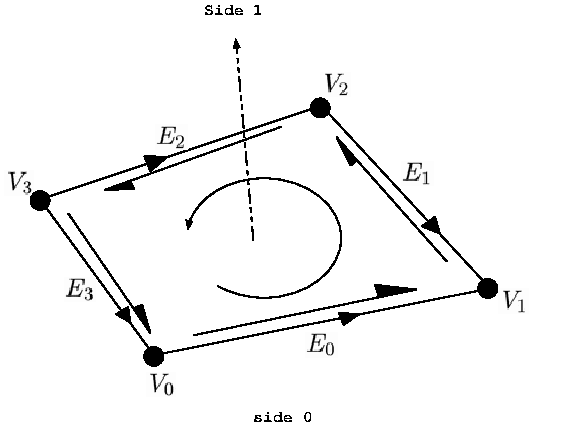
\includegraphics[scale=1.0]{figures/face_def} 
  \caption{Face definition}
  \label{fig:face_def}
  \end{center}
\end{figure}


\item[]\textbf{\textit{Set\_ptr} MF\_Edges(\textit{MFace\_ptr} mface,
    \textit{int} dir, \textit{MVertex\_ptr} mvert):} Return the
  ordered set of edges of the face. The edges are ordered in the ccw
  while looking down the face 'normal' if dir is 1 and in the cw if
  dir is 0. If 'mvert' is specified, the edge set is reordered so that
  the first edge in the set contains this vertex. More precisely, if
  'dir' is 1, and the first edge is 'e' used in the face in direction
  'd', then \textbf{ME\_Vertex(e,!d)} = mvert. With reference to
  Figure~\ref{fig:face_def}, the edges of the face in the ccw direction or
  'dir' = 1 are ${E_0,E_1,E_2,E_3}$ and in the opposite dir are
  ${E_3,E_2,E_1,E_0}$. If 'mvert' or the starting vertex is specified
  as $V_2$, the edge set in ccw direction or 'dir' = 1 is
  ${E_2,E_3,E_0,E_1}$ and in the opposite direction is
  ${E_1,E_0,E_3,E_2}$.

\item[]\textbf{\textit{Set\_ptr} MF\_AdjFaces(\textit{MFace\_ptr} mface):}
Set of adacent faces of a face. This operator is relevant only in
planar or surface surface meshes, i.e., for boundary faces not
connected to any regions.

\item[]\textbf{\textit{int} MF\_EdgeDir(\textit{MFace\_ptr} mface,
\textit{MEdge\_ptr} medge):} Returns the direction in which the face
uses the given edge. If the faces use the edge in the positive direction,
the function returns 1; otherwise it returns 0.

\item[]\textbf{\textit{int} MF\_EdgeDir\_i(\textit{MFace\_ptr} mface,
\textit{int} i):} Returns the direction in which the face uses its i'th
edge. If the face uses the edge in the positive direction the function
returns 1; otherwise it returns 0;

\item[]\textbf{\textit{int} MF\_UsesEntity(\textit{MFace\_ptr} mface,
\textit{MEntity\_ptr} mentity, \textit{int} type):} Check if the face
uses the given lower dimension entity, 'mentity'. The type of the
entity is specified by the 'etype' variable. For a face, a lower
dimensional entity can be a vertex or an edge. If the face uses the
vertex or the edge, the function returns 1; otherwise it returns 0. If
any other type of entity is specified, the function returns 0.

\item[]\textbf{\textit{Set\_ptr} MF\_Regions(\textit{MFace\_ptr} mface):}
Return the set of regions connected to the face. If the face is not
used by any regions, the function returns NULL to indicate that the
set is empty. If not the set may contain one or two regions.

\item[]\textbf{\textit{MRegion\_ptr} MF\_Region(\textit{MFace\_ptr} mface,
\textit{int} side):} Returns the region on the specified side of the
face. The positive side of the face (side = 1) is the side towards
which the face normal points. The negative side of the face (side = 0)
is the opposite side.

\item[]\textbf{\textit{void} MF\_Coords(\textit{MFace\_ptr} mface,
\textit{int} *n, double (*xyz)[3], \textit{int} dir):} Returns the
coordinates of the face vertices in an array along with the number of
vertices. If 'dir' is 1, the coordinates are returned with a  ccw
ordering while looking down the face normal; if 'dir' is 0, they are
returned with a cw ordering (See Figure~\ref{fig:face_def}).
\end{description}

\newpage
\subsection{Mesh Region Object}

\begin{description}
\item[]\textbf{\textit{MRegion\_ptr} MR\_New(\textit{Mesh\_ptr} mesh):}
Create a new region object. No topological information is embedded in
the region when it is created. The region only knows which mesh it
belongs to. The ID of the region is set by this function.

\item[]\textbf{\textit{void} MR\_Delete(\textit{MRegion\_ptr} mregion):}
Delete the region. Deletes all topological information embedded in the
edge.

\item[]\textbf{\textit{void} MR\_Set\_GEntity(\textit{MRegion\_ptr} mregion,
GEntity\_ptr gent):} Set the geometric model entity on which the edge
is classified.

\item[]\textbf{\textit{void} MR\_Set\_GEntDim(\textit{MRegion\_ptr} mregion,
\textit{int} gdim):} Set the dimension of the geometric model entity on
which the edge is classified.

\item[]\textbf{\textit{void} MR\_Set\_GEntID(\textit{MRegion\_ptr} mregion,
\textit{int} gid):} Set the ID of the geometric model entity on which
the edge is classified.

\item[]\textbf{\textit{void} MR\_Set\_ID(\textit{MRegion\_ptr} mregion,
\textit{int} id):} Explicitly set ID of an edge and overwrite the ID
set by the \textbf{MR\_New} function. Does not check for duplication
of region IDs.

\item[]\textbf{\textit{void} MR\_Set\_Faces(\textit{MRegion\_ptr} mregion,
\textit{int} nf, \textit{MFace\_ptr} *mfaces, \textit{int} *dirs):} Set
the faces of the region along with their directions. The
\textit{unordered} set of faces and their directions are passed in
through arrays along with the number of faces. If the normal of the
face points out of the region, the associated direction to be passed
in is 1; otherwise it is 0. This function is only relevant for full
representations in MSTK.

\item[]\textbf{\textit{void} MR\_Set\_Vertices(\textit{MRegion\_ptr}
mregion, \textit{int} nv, \textit{MVertex\_ptr} *mvertices):} Set the
vertices of the region. This function is relevant for reduced
representations only. For standard elements, the vertices must be
ordered as indicated in Appendix~\ref{app:reg_conventions}. This
function does not apply for defining general regions since there
cannot be any implicit ordering.

\item[]\textbf{\textit{void} MR\_Replace\_Face(\textit{MRegion\_ptr}
mregion, \textit{MFace\_ptr} mface, \textit{MFace\_ptr} nuface,
\textit{int} dir):} Replace a face of the region with another edge. The
direction in which the new face is used in the region must also be
supplied. This function is only relevant for full representations in
MSTK.

\item[]\textbf{\textit{void} MR\_Replace\_Vertex(\textit{MRegion\_ptr}
mregion, \textit{MVertex\_ptr} mvertex, \textit{MVertex\_ptr}
nuvertex):} Replace a vertex of a region with another vertex. This
function is relevant only for reduced representations in MSTK.

\item[]\textbf{\textit{void} MR\_Replace\_Face\_i(\textit{MRegion\_ptr}
mregion, \textit{int} i, \textit{MFace\_ptr} mface, \textit{int} dir):}
Replace the i'th face in the region with another face.The direction in
which the new face is used in the region must also be supplied. This
function is only relevant for full representations in MSTK.

\item[]\textbf{\textit{void} MR\_Replace\_Vertex\_i(\textit{MRegion\_ptr}
mregion, \textit{int} i, \textit{MVertex\_ptr} mvertex):} Replace the
i'th vertex of the region with another vertex. This function is only
relevant for reduced representations in MSTK.


\item[]\textbf{\textit{Mesh\_ptr} MR\_Mesh(\textit{MRegion\_ptr} mregion):}
Returns the mesh that the region belongs to.

\item[]\textbf{\textit{int} MR\_ID(\textit{MRegion\_ptr} mregion):} Returns
the ID of the region. Returns 0 if not known.

\item[]\textbf{\textit{int} MR\_GEntDim(\textit{MRegion\_ptr} mregion):}
Returns the dimension of the geometric model entity the region is
classified on. Always returns 3 since a mesh region can be classified
only on a model region.

\item[]\textbf{\textit{int} MR\_GEntID(\textit{MRegion\_ptr} mregion):}
Returns the ID of the geometric model entity that the region is
classified on. Returns 0 if not known.

\item[]\textbf{\textit{GEntity\_ptr} MR\_GEntity(\textit{MRegion\_ptr}
  mregion):} Returns a pointer or handle to the geometric model entity
  that the vertex is classified on. Returns NULL if this information
  is not known.

\item[]\textbf{\textit{int} MR\_Num\_Vertices(\textit{MRegion\_ptr}
mregion):} Returns the number of vertices of a region.

\item[]\textbf{\textit{int} MR\_Num\_Edges(\textit{MRegion\_ptr} mregion):}
Returns the number of edges of a region.

\item[]\textbf{\textit{int} MR\_Num\_Faces(\textit{MRegion\_ptr} mregion):}
Returns the number of faces of a region.

\item[]\textbf{\textit{int} MR\_Num\_AdjRegions(\textit{MRegion\_ptr}
mregion):} Returns the number of adjacent regions of a region, i.e.,
regions sharing a face with this region.

\item[]\textbf{\textit{Set\_ptr} MR\_Vertices(\textit{MRegion\_ptr}
mregion):} Returns the set of vertices of a region. For standard
elements the vertices are ordered as indicated in
Appendix~\ref{app:reg_conventions}. For non-standard elements the set
is unordered.

\item[]\textbf{\textit{Set\_ptr} MR\_Edges(\textit{MRegion\_ptr} mregion):}
Return the \underline{unordered} set of edges of a region. 

\item[]\textbf{\textit{Set\_ptr} MR\_Faces(\textit{MRegion\_ptr} mregion):}
Returns the set of faces of a region.

\item[]\textbf{\textit{Set\_ptr} MR\_AdjRegions(\textit{MRegion\_ptr}
mregion):} Returns the set of adjacent regions of a region, i.e.,
regions sharing a face with this region. The set is not ordered.

\item[]\textbf{\textit{int} MR\_FaceDir(\textit{MRegion\_ptr} mregion,
\textit{MFace\_ptr} mface):} Returns the direction in which the region
uses the given face. Returns 1 if the face normal points out of the
region and returns 0 if the face normal points into the region.

\item[]\textbf{\textit{int} MR\_FaceDir\_i(\textit{MRegion\_ptr} mregion,
\textit{int} i):} Returns the direction in which the region uses the
i'th face. Returns 1 if the face normal points out of the region and
returns 0 if the face normal points into the region.

\item[]\textbf{\textit{int} MR\_UsesEntity(\textit{MRegion\_ptr} mregion,
\textit{MEntity\_ptr} ment, \textit{int} type):} Check if the region
uses the given lower dimension entity, 'mentity'. The type of the
entity is


\item[]\textbf{\textit{void} MR\_Coords(\textit{MRegion\_ptr} mregion,
\textit{int} *n, double (*xyz)[3]):} Returns the coordinates of the
region vertices in an array along with the number of vertices. For
standard elements, the ordering is as given in
Appendix~\ref{app:reg_conventions}. For non-standard elements, the
ordering is arbitrary.
\end{description}



\newpage
\subsection{Generic Entity Object}

The following functions operate on generic mesh entities of type
\textit{MEntity\_ptr}. This implies that variables of type
\textit{MVertex\_ptr}, \textit{MEdge\_ptr}, \textit{MFace\_ptr},
\textit{MRegion\_ptr} can all be passed in place of
\textit{MEntity\_ptr} variables in the following functions.

\begin{description}
%%  \textit{void} MEnt\_Set\_GEntity(\textit{MEntity\_ptr} mentity, GEntity\_ptr gent);
%%
%%  \textit{void} MEnt\_Set\_GEntDim(\textit{MEntity\_ptr} mentity, \textit{int} gdim);
%%
%%  \textit{void} MEnt\_Set\_ID(\textit{MEntity\_ptr} mentity, \textit{int} id);

  
\item[]\textbf{\textit{int} MEnt\_ID(\textit{MEntity\_ptr} mentity):} Returns
the ID of a generic entity.

\item[]\textbf{\textit{int} MEnt\_Dim(\textit{MEntity\_ptr} mentity):}
Returns the topological dimension or type of generic entity.

\item[]\textbf{\textit{Mesh\_ptr} MEnt\_Mesh(\textit{MEntity\_ptr} mentity):}
Returns the mesh that the entity belongs to.

\item[]\textbf{\textit{int} MEnt\_GEntDim(\textit{MEntity\_ptr} mentity):}
Returns the dimension of the geometric model entity that the entity is
classified on.

\item[]\textbf{\textit{GEntity\_ptr} MEnt\_GEntity(\textit{MEntity\_ptr} mentity):}
Returns a pointer or handle to geometric model entity that the entity
is classified on.
\end{description}




\newpage
\subsection{Entity Marks}

Entity marks or markers are a way of tagging entities. Such
functionality is useful in algorithms which must keep track of
processed entities to avoid duplication of work. An example of such an
operation is creating a union of entity sets while extracting upward
adjacency information such as the regions connected to an edge.

\begin{description}
\item[]\textbf{\textit{int} MSTK\_GetMarker():} Returns a unique marker ID
which may be used to tag entities.

\item[]\textbf{\textit{void} MEnt\_Mark(\textit{MEntity\_ptr} ent, \textit{int} mkr):} Mark an entity with the given marker 'mkr'.

\item[]\textbf{\textit{int} MEnt\_IsMarked(\textit{MEntity\_ptr} ent, \textit{int} mkr):} Check if an entity is marked with the given marker 'mkr'.

\item[]\textbf{\textit{void} MEnt\_Unmark(\textit{MEntity\_ptr} ent, \textit{int} mkr):} Unmark an entity with respect to the given marker 'mkr'

\item[]\textbf{\textit{void} Set\_Mark(\textit{Set\_ptr} list, \textit{int} mkr):} Mark a set of entities with given marker.

\item[]\textbf{\textit{void} Set\_Unmark(\textit{Set\_ptr} list, \textit{int} mkr):}
Unmark a set of entities with respect to the given marker.

\item[]\textbf{\textit{void} MSTK\_FreeMarker(\textit{int} mkr):} Release the
marker ID given by \textbf{MSTK\_GetMarker()} so that it can be
reused. Care must be taken to unmark all entities marked with this
marker ID before releasing it. If not, subsequent operations with
reassigned marker will find a tag on some entities and mistake them
for being processed.
\end{description}




\newpage
\subsection{Mesh Modification}

\begin{description}

\item[]\textbf{\textit{int} ME\_Swap2D(\textit{MEdge\_ptr} e,
\textit{MEdge\_ptr} *enew, \textit{MFace\_ptr} fnew[2]):} Swap an edge
in a triangular mesh. No checks are performed for topological or
geometric validity.

\item[]\textbf{\textit{MFace\_ptr} MFs\_Join(\textit{MFace\_ptr} f1,
\textit{MFace\_ptr} f2, \textit{MEdge\_ptr} e):} Join two faces along
common edge and create new face by eliminating the common edge as
shown in Figure~\ref{fig:MFs_Join}. If 'f1' has 'n1' edges and 'f2'
has 'n2' edges, then the new face has ('n1'+'n2'-2) edges.

\end{description}

\begin{figure}[!h]
  \begin{center}
    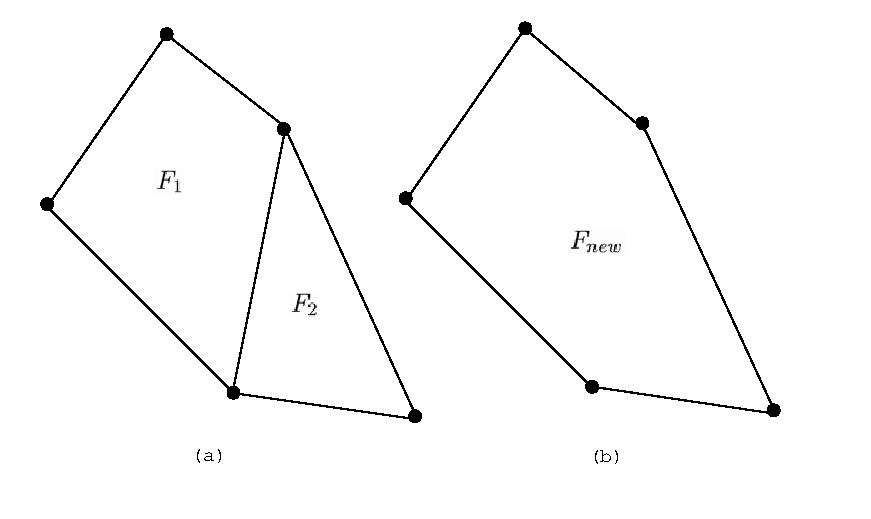
\includegraphics[scale=1.0]{figures/MFs_Join}
    
    \caption{Joining two faces (a) Two faces $F_1$ and $F_2$ sharing a
      common edge (b) New pentagonal face $F_{new}$ created by
      eliminating the common edge.  }
    \label{fig:MFs_Join}
  \end{center}
\end{figure}

\newpage
\subsection{Utilities}
  
\begin{description}
  
\item[]\textbf{\textit{void} MSTK\_Report(\textit{char} *module,
  \textit{char} *message, \textit{ErrType} severity):} Error handler
  for MSTK. 'module' is the name of the function in which the error
  occurs. 'message' is the error message and is recommended to be less
  than 1024 characters in length. 'severity' is an error code and can
  be MESSG, WARN, ERROR or FATAL. If the error code is FATAL, the
  program will quit after printing the error. If the same message is
  repeated successively, then the message is printed only the first
  time.

\item[]\textbf{\textit{void} Set\_PrintID(\textit{Set\_ptr} l):} Debugging
utility to print the IDs of the entities in a set.

\item[]\textbf{\textit{void} MV\_Print(\textit{MVertex\_ptr} v, int
    lev):} Debugging utility to print information about a mesh vertex,
  \textbf{v}. The argument \textbf{lev} controls the level of detail
  of the information printed. \textbf{lev} = 0 prints the minimum
  information, i.e., vertex pointer, its ID and its coordinates. If
  \textbf{lev} = 1, the function prints classification information for
  the vertex (if available), i.e., ID and dimension of the model
  entity that the vertex is on. If \textbf{lev} $>$ 1, then upward
  detailed adjacency information is also printed for the vertex, i.e.,
  information is printed about the edges, faces and regions connected
  to the vertex.
  
\item[]\textbf{\textit{void} ME\_Print(\textit{MEdge\_ptr} e, int
    lev):} Debugging utility to print information about a mesh edge,
  \textbf{e}. The argument \textbf{lev} controls the level of detail
  of the information printed. \textbf{lev} = 0 prints the minimum
  information, i.e., edge pointer, its ID and the IDs of its two
  vertices. If \textbf{lev} = 1, the function prints classification
  information for the edge (if available), i.e., ID and dimension of
  the model entity that the edge is on. Also, more detailed vertex
  information printed in this case. If \textbf{lev} $>$ 1, the
  function prints detailed upward adjacency information for the edge,
  i.e., information is printed about the faces and regions connected
  to the edge.
    
  \item[]\textbf{\textit{void} MF\_Print(\textit{MFace\_ptr} f, int
      lev):} Debugging utility to print information about a mesh face,
    \textbf{f}. The argument \textbf{lev} controls the level of detail
    of the information printed. \textbf{lev} = 0 prints the minimum
    information, i.e., the face pointer and its ID. If \textbf{lev} =
    1, the function prints classification information for the edge (if
    available), i.e., ID and dimension of the model entity that the
    face is on. Also, a signed list of the edges of the face is
    printed.  If \textbf{lev} $>$ 1, the function prints detailed
    downward and upward adjacency information for the face, i.e.,
    information is printed about the edges and vertices of the face,
    and about the regions connected to the face.
    
  \item[]\textbf{\textit{void} MR\_Print(\textit{MRegion\_ptr} r, int
      lev):} Debugging utility to print information about a mesh
    region, \textbf{r}. The argument \textbf{lev} controls the level
    of detail of the information printed. \textbf{lev} = 0 prints the
    minimum information, i.e., region pointer and its ID. If
    \textbf{lev} = 1, the function prints classification information
    for the region (if available), i.e., ID of the model entity that
    the region is on. Also, a signed list of the faces of the region
    is printed. If \textbf{lev} $>$ 1, the function prints detailed
    downward adjacency information for the region, i.e., information
    is printed about the faces, edges and vertices forming the region.



\end{description}

\newpage
\appendix

\section{Mesh Representation Types  in MSTK}
\label{app:reptypes}

\begin{figure}[!h]
%  \begin{center}
    \begin{minipage}{2.525in}
      \begin{center}
        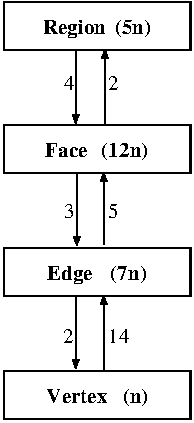
\includegraphics[scale=0.9]{figures/repF1} \\
        Representation F1
      \end{center}
    \end{minipage}\hfill%
    \begin{minipage}{2.525in}
      \begin{center}
        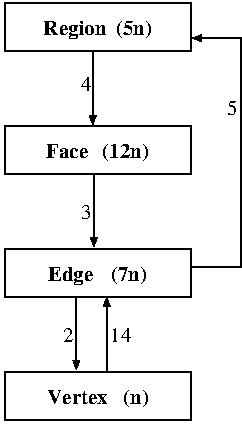
\includegraphics[scale=0.9]{figures/repF4} \\
        Representation F4
      \end{center}
    \end{minipage}
    \vspace{5em}

    \begin{minipage}{1.75in}
      \begin{center}
        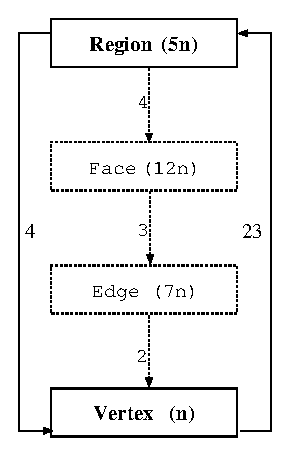
\includegraphics[scale=0.9]{figures/repR1} \\
        Representation R1
      \end{center}
    \end{minipage}
    \begin{minipage}{1.75in}
      \begin{center}
        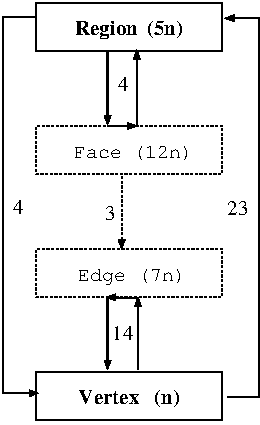
\includegraphics[scale=0.9]{figures/repR2} \\
        Representation R2
      \end{center}
    \end{minipage}
    \begin{minipage}{1.75in}
      \begin{center}
        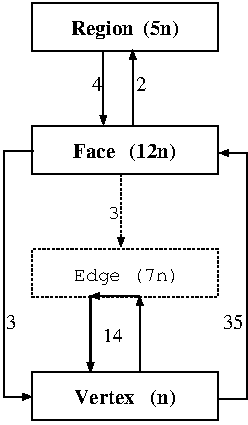
\includegraphics[scale=0.9]{figures/repR4} \\
        Representation R4
      \end{center}
    \end{minipage}
%  \end{center}
\end{figure}

\newpage
\section{Conventions for Vertex, Edge Numbering in Standard Region Types}
\label{app:reg_conventions}

\begin{figure}[!h]
  \begin{center}
    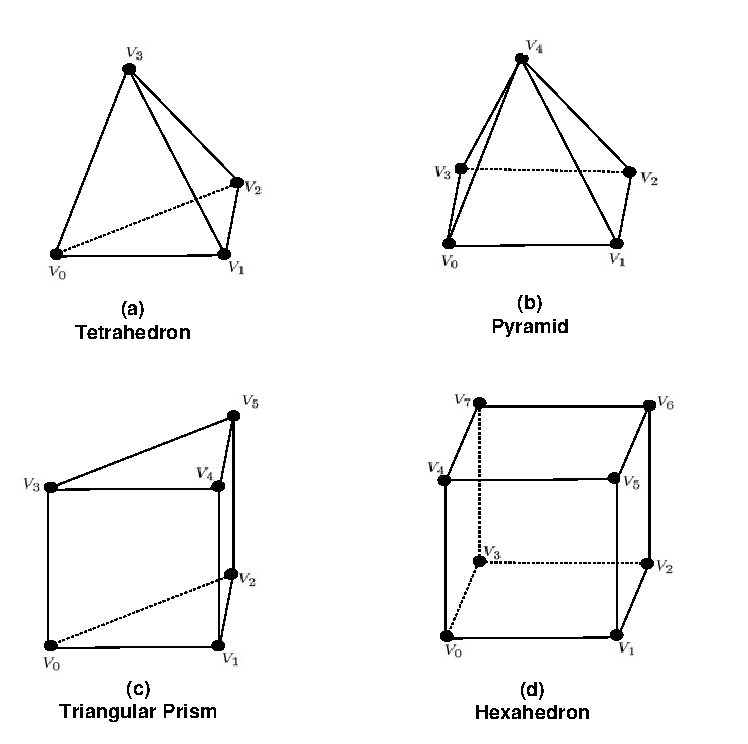
\includegraphics[scale=1.0]{figures/reg_conventions}
  \end{center}
\end{figure}

\newpage
\section{MSTK File Format}
\label{app:file_format}

\subsection{MSTK ASCII File Format}

\begin{verse}
\# \textit{This is a comment} \\
\# \textit{The string ``MSTK'' and File version number (1.0)} \\
\vspace{1ex}
 
MSTK Ver %
\vspace{1ex}

\# \textit{char *reptype - Type of representation} \\  
\# \textit{\textit{int} NV, NE, NF, NR - Number of vertices, edges, face, regions} \\
\vspace{1ex}

RepType \hspace{0.5ex} NV \hspace{0.5ex} NE \hspace{0.5ex} NF \hspace{0.5ex} NR \\
\hspace{2ex}

\# \textit{\textbf{VERTEX INFO}} \\
\# \textit{Each record has} \\
\# \textit{double X,Y,Z Coordinates} \\
\# \textit{\textit{int} Mdim - Topological type or dimension of model entity that} \\
\# \textit{\hspace{4.7em} the vertex is on} \\
\# \textit{\textit{int} Mid - ID of model entity the vertex is on} \\
\# \textit{Mdim and Mid can be -1 and 0 resp. if model info. is absent} 
\vspace{1ex}

X\_Coord \hspace{0.5ex} Y\_Coord \hspace{0.5ex} Z\_Coord \hspace{0.5ex} Mdim \hspace{0.5ex} Mid \\
X\_Coord \hspace{0.5ex} Y\_Coord \hspace{0.5ex} Z\_Coord \hspace{0.5ex} Mdim \hspace{0.5ex} Mid \\
. . . \\
\# \textit{Repeated NV times}
\vspace{2ex}

\# \textit{\textbf{EDGE INFO} - present only if NE $\ne$ 0} \\
\# \textit{Keyword 'edges' followed by edge records}
\# \textit{Each edge record has} \\
\# \textit{\textit{int} Vid\_1, Vid\_2  - IDs of first, second vertex of edge} \\
\# \textit{\textit{int} Mdim, Mid}
\vspace{1ex}

edges
Vid\_1 \hspace{0.5ex} Vid\_2 \hspace{0.5ex} Mdim \hspace{0.5ex} Mid \\
Vid\_1 \hspace{0.5ex} Vid\_2 \hspace{0.5ex} Mdim \hspace{0.5ex} Mid \\
. . . \\
\# \textit{Repeated NEdges times}
\vspace{2ex}

\newpage
\# \textit{\textbf{FACE INFO} - present only if NF $\ne$ 0} \\
\# \textit{Keyword 'faces'}
\# \textit{char *FLtype: Keyword for lower order entity describing faces} \\
\# \textit{Values: Vertex, Edge (case insensitive), e.g. VeRteX or EDGE} \\
\vspace{1ex}

faces FLtype 
\vspace{1ex}

\# \textit{If face described by vertices, then each face record has} \\
\# \textit{\textit{int} NFV - Number of face vertices} \\
\# \textit{\textit{int} Vid\_1 - ID of first vertex of face} \\
\# \textit{\textit{int} Vid\_2 - ID of second vertex of face} \\
\# . . . \\
\# \textit{\textit{int} Vid\_1 - ID of NFV'th vertex of face} \\
\# \textit{\textit{int} Mdim, Mid} 
\vspace{1ex}

NFV \hspace{0.5ex} Vid\_1 \hspace{0.5ex} Vid\_2 \hspace{0.5ex} ... \hspace{0.5ex} Vid\_NFV \hspace{0.5ex} Mdim \hspace{0.5ex} Mid \\
NFV \hspace{0.5ex} Vid\_1 \hspace{0.5ex} Vid\_2 \hspace{0.5ex} ... \hspace{0.5ex} Vid\_NFV \hspace{0.5ex} Mdim \hspace{0.5ex} Mid \\
. . . \\
\# \textit{Repeated NFaces times}
\vspace{2ex}\vspace{1ex}

\# \textit{If face described by edges, then each face record has} \\
\# \textit{\textit{int} NFE - Number of face edges} \\
\# \textit{\textit{int} $\pm$Eid\_1 - signed ID of first edge of face} \\
\# \textit{\textit{int} $\pm$Eid\_2 - signed ID of second edge of face} \\
\# . . . \\
\# \textit{\textit{int} $\pm$Eid\_NFE - signed ID of NFE'th edge of face} \\
\# \textit{\textit{int} Mdim, Mid} \\
\# \\
\# \textit{if sign of edge is +, face uses edge in direction it was defined} \\
\# \textit{if sign of edge is -, face uses edge in opposite direction} \\
\vspace{1ex}

NFE \hspace{0.5ex} $\pm$Eid\_1 \hspace{0.5ex} $\pm$Eid\_2 \hspace{0.5ex} ... \hspace{0.5ex} $\pm$Eid\_NFE \hspace{0.5ex} Mdim Mid \\
NFE \hspace{0.5ex} $\pm$Eid\_1 \hspace{0.5ex} $\pm$Eid\_2 \hspace{0.5ex} ... \hspace{0.5ex} $\pm$Eid\_NFE \hspace{0.5ex} Mdim Mid \\
. . . \\
\# \textit{Repeated NFaces times}
\vspace{2ex}\vspace{1ex}


\# \textit{\textbf{REGION INFO} - present only if NR $\ne$ 0} \\
\# \textit{Keyword 'regions'}
\# \textit{char *RLtype - keyword for lower order entity describing region} \\
\# \textit{Values: Vertex, Face (case insensitive), e.g. VERtex or faCE}
\vspace{1ex}

regions RLtype
\vspace{1ex}

\# \textit{if region described by vertices, then each region record has} \\
\# \textit{\textit{int} NRV - Number of region vertices} \\
\# \textit{\textit{int} Vid\_1 - ID of first vertex of region} \\
\# \textit{\textit{int} Vid\_2 - ID of second vertex of region} \\
\# . . . \\
\# \textit{\textit{int} Vid\_NFE - ID of NRV'th vertex of region} \\
\# \textit{\textit{int} Mid, (NOTE: Mdim is not specified, since it has to be 3)}
\vspace{1ex}

NRV \hspace{0.5ex} Vid\_1 \hspace{0.5ex} Vid\_2 \hspace{0.5ex} ... \hspace{0.5ex} Vid\_NRV \hspace{0.5ex} Mid \\
NRV \hspace{0.5ex} Vid\_1 \hspace{0.5ex} Vid\_2 \hspace{0.5ex} ... \hspace{0.5ex} Vid\_NRV \hspace{0.5ex} Mid \\
. . . \\
\# \textit{Repeat NR times} 
\vspace{3ex}

\# \textit{if region described by faces, then each region record has} \\
\# \textit{\textit{int} NRF - Number of region faces} \\
\# \textit{\textit{int} Fid\_1 - signed ID of first face of region} \\
\# \textit{\textit{int} Fid\_2 - signed ID of second face of region} \\
\# . . . \\
\# \textit{\textit{int} Fid\_NRF - signed ID of NRF'th face of region} \\
\# \textit{\textit{int} Mdim, Mid} \\
\#  \\
\# \textit{if sign of face is +, face normal points out of region} \\
\# \textit{if sign of edge is -, face normal points into region}
\vspace{1ex}

NRF \hspace{0.5ex} $\pm$Fid\_1 \hspace{0.5ex} $\pm$Fid\_2 \hspace{0.5ex} ... \hspace{0.5ex} $\pm$Fid\_NRF \hspace{0.5ex} Mid \\
NRF \hspace{0.5ex} $\pm$Fid\_1 \hspace{0.5ex} $\pm$Fid\_2 \hspace{0.5ex} ... \hspace{0.5ex} $\pm$Fid\_NRF \hspace{0.5ex} Mid \\
. . . \\
\# \textit{Repeated NR times} 
\vspace{2ex}

\# \textit{\textbf{NOT IMPLEMENTED}}

\# \textit{\textbf{VERTEX ATTRIBUTES}} \\
\# \textit{\textit{int} NVA - Number of Vertex attributes} \\
\# \\
\# \textit{char *VA\_name\_1 - Name of first vertex attribute} \\
\# \textit{\textit{int} VA\_type\_1 - Type of first vertex attribute} \\
\# \textit{\textit{int} VA\_dim\_1 - Dimension of first vertex attribute} \\
\# \\
\# \textit{char *VA\_name\_2 - Name of second vertex attribute} \\
\# \textit{\textit{int} VA\_type\_2 - Type of second vertex attribute} \\
\# \textit{\textit{int} VA\_dim\_2 - Dimension of first vertex attribute} \\
\# \\
\# . . .\\
\# \\
\# \textit{char *VA\_name\_NVA - Name of NVA'th vertex attribute} \\
\# \textit{\textit{int} VA\_type\_NVA - Type of NVA'th vertex attribute} \\
\# \textit{\textit{int} VA\_dim\_NVA - Dimension of NVA'th vertex attribute} \\
\# \\
\# \textit{VA\_type can be 1 (int), 2 (double), 3 (string)} \\
\# \textit{VA\_dim = 1 for scalars, VA\_dim = length of vector for vector} \\
\# \textit{VA\_dim can only be 1 when VA\_type is string}
\vspace{1ex}

NVA \hspace{0.5ex} \\
VA\_name\_1 \hspace{0.5ex} VA\_type\_1 \hspace{0.5ex} VA\_dim\_1 \\ 
VA\_name\_2 \hspace{0.5ex} VA\_type\_2 \hspace{0.5ex} VA\_dim\_2 \\
. \\
VA\_dim\_NVA \hspace{0.5ex} VA\_type\_NVA \hspace{0.5ex} VA\_dim\_2  
\vspace{1ex}

\# \textit{For each vertex attribute record, set of attribute values} \\
\# \textit{E.G., there are 3 attributes for each vertex:} \\
\# \textit{a scalar int, a vector of 3 doubles and a string}

VA\_\textit{int} \hspace{0.5ex} VA\_double\_1 \hspace{0.5ex} VA\_double\_2 \hspace{0.5ex} VA\_double\_3 \hspace{0.5ex} VA\_string \\
VA\_\textit{int} \hspace{0.5ex} VA\_double\_1 \hspace{0.5ex} VA\_double\_2 \hspace{0.5ex} VA\_double\_3 \hspace{0.5ex} VA\_string \\
. \\
. \\
. \\
\# \textit{Repeated NV times}
\vspace{2ex}

\newpage
\# \textit{\textbf{EDGE ATTRIBUTES}} \\
\# \textit{Similar to Vertex attribute description}
\vspace{1ex}

NEA \hspace{0.5ex} \\
EA\_name\_1 \hspace{0.5ex} EA\_type\_1 \hspace{0.5ex} EA\_dim\_1 \\ 
EA\_name\_2 \hspace{0.5ex} EA\_type\_2 \hspace{0.5ex} EA\_dim\_2 \\
. \\
EA\_dim\_NEA \hspace{0.5ex} EA\_type\_NEA \hspace{0.5ex} EA\_dim\_2  
\vspace{1ex}

\# \textit{For each edge attribute record, set of attribute values} \\
\# \textit{E.G., a scalar int, a scalar double and a string}
\vspace{1ex}

EA\_\textit{int} \hspace{0.5ex} EA\_double \hspace{0.5ex} EA\_string \\
EA\_\textit{int} \hspace{0.5ex} EA\_double \hspace{0.5ex} EA\_string \\
. . . \\
\# \textit{Repeated NE times}
\vspace{2ex}

\# \textit{\textbf{FACE ATTRIBUTES}} \\
\# \textit{Similar to Vertex attribute description}
\vspace{1ex}

NFA \hspace{0.5ex} \\
FA\_name\_1 \hspace{0.5ex} FA\_type\_1 \hspace{0.5ex} FA\_dim\_1 \\ 
FA\_name\_2 \hspace{0.5ex} FA\_type\_2 \hspace{0.5ex} FA\_dim\_2 \\
. \\
FA\_dim\_NFA \hspace{0.5ex} FA\_type\_NEA \hspace{0.5ex} FA\_dim\_2  
\vspace{1ex}

\# \textit{For each face attribute record, set of attribute values} \\
\# \textit{E.G., a vector of 2 doubles and a string}
\vspace{1ex}

FA\_double\_1 \hspace{0.5ex} FA\_double\_2 \\
FA\_double\_1 \hspace{0.5ex} FA\_double\_2 \\
. . . \\
\# \textit{Repeated NF times}
\vspace{2ex}

\newpage
\# \textit{\textbf{REGION ATTRIBUTES}} \\
\# \textit{Similar to Vertex attribute description}
\vspace{1ex}

NRA \hspace{0.5ex} \\
RA\_name\_1 \hspace{0.5ex} RA\_type\_1 \hspace{0.5ex} RA\_dim\_1 \\ 
RA\_name\_2 \hspace{0.5ex} RA\_type\_2 \hspace{0.5ex} RA\_dim\_2 \\
. \\
RA\_dim\_NRA \hspace{0.5ex} RA\_type\_NRA \hspace{0.5ex} RA\_dim\_NRA 
\vspace{1ex}

\# \textit{For each Region attribute record, set of attribute values} \\
\# \textit{E.G., a vector of 3 ints}
\vspace{1ex}

RA\_int\_1 \hspace{0.5ex} RA\_int\_2 \hspace{0.5ex} RA\_int\_3 \\
RA\_int\_1 \hspace{0.5ex} RA\_int\_2 \hspace{0.5ex} RA\_int\_3 \\
. . .\\
\# \textit{Repeated NR times}
\vspace{2ex}

\end{verse}

\newpage



\end{document}
